\documentclass{standalone}
\usepackage{tikz}
\usetikzlibrary{patterns, positioning}


\begin{document}
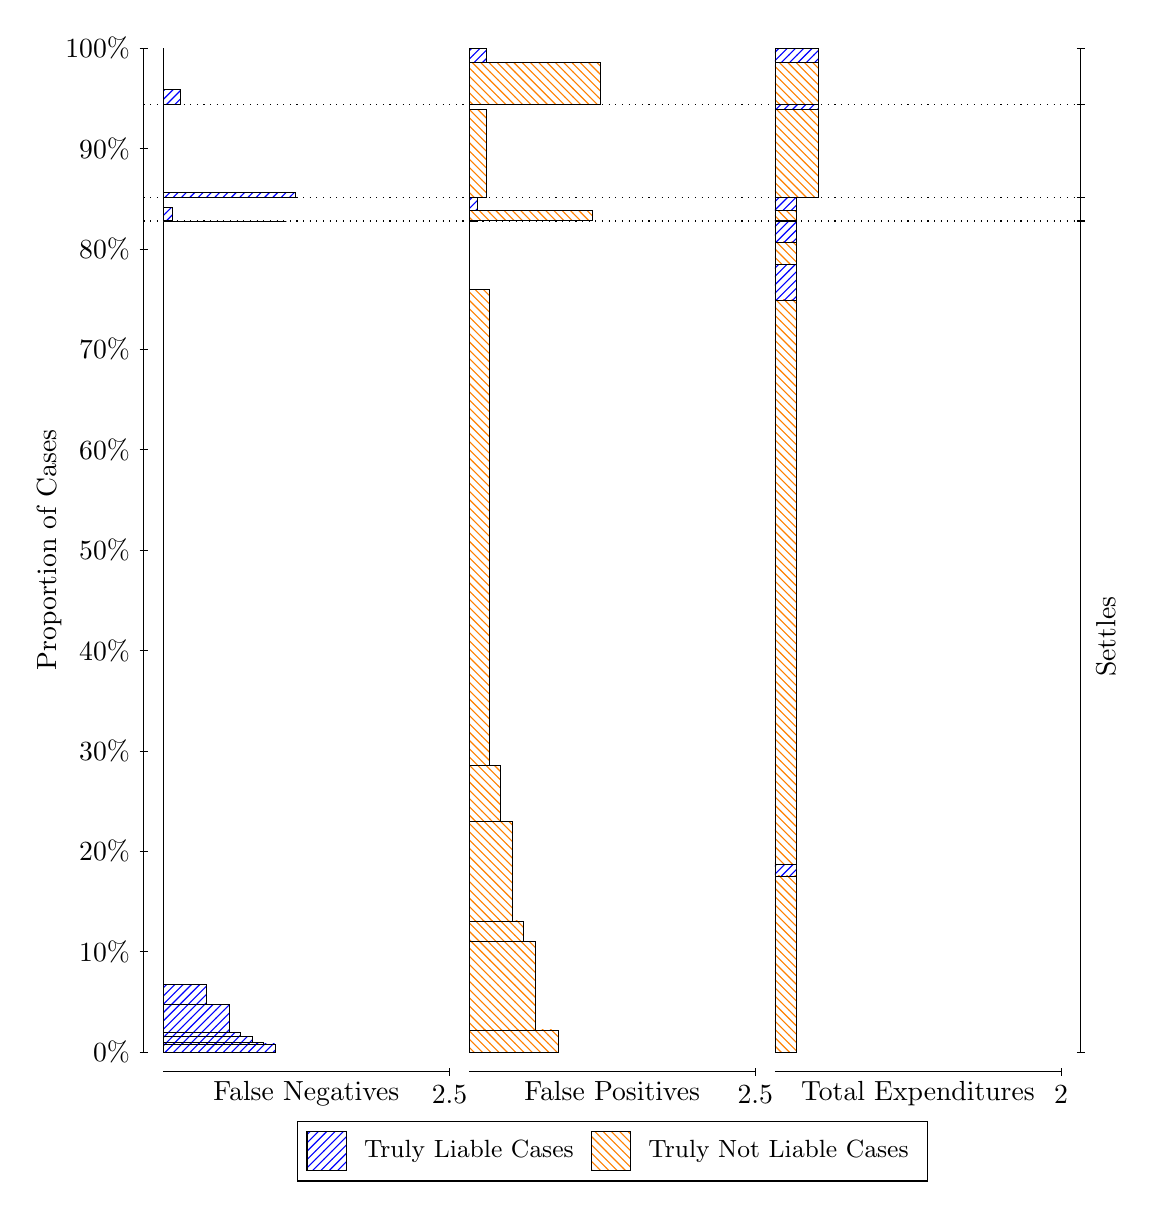
\begin{tikzpicture}
\draw[black, very thin] (1.5,1.75) -- (1.5,14.5);
\node[rotate=90, text=black, anchor=center] at (0.3, 8.125) {Proportion of Cases};
\draw[black, very thin] (1.45,1.75) -- (1.55,1.75);
\node[text=black, anchor=east] at (1.45, 1.75) {0\%};
\draw[black, very thin] (1.45,3.025) -- (1.55,3.025);
\node[text=black, anchor=east] at (1.45, 3.025) {10\%};
\draw[black, very thin] (1.45,4.3) -- (1.55,4.3);
\node[text=black, anchor=east] at (1.45, 4.3) {20\%};
\draw[black, very thin] (1.45,5.575) -- (1.55,5.575);
\node[text=black, anchor=east] at (1.45, 5.575) {30\%};
\draw[black, very thin] (1.45,6.85) -- (1.55,6.85);
\node[text=black, anchor=east] at (1.45, 6.85) {40\%};
\draw[black, very thin] (1.45,8.125) -- (1.55,8.125);
\node[text=black, anchor=east] at (1.45, 8.125) {50\%};
\draw[black, very thin] (1.45,9.4) -- (1.55,9.4);
\node[text=black, anchor=east] at (1.45, 9.4) {60\%};
\draw[black, very thin] (1.45,10.675) -- (1.55,10.675);
\node[text=black, anchor=east] at (1.45, 10.675) {70\%};
\draw[black, very thin] (1.45,11.95) -- (1.55,11.95);
\node[text=black, anchor=east] at (1.45, 11.95) {80\%};
\draw[black, very thin] (1.45,13.225) -- (1.55,13.225);
\node[text=black, anchor=east] at (1.45, 13.225) {90\%};
\draw[black, very thin] (1.45,14.5) -- (1.55,14.5);
\node[text=black, anchor=east] at (1.45, 14.5) {100\%};

\draw[black, very thin] (13.4,1.75) -- (13.4,14.5);
\draw[black, very thin] (13.35,1.75) -- (13.45,1.75);
\node[anchor=west] at (13.35, 1.75) {};
\draw[black, very thin] (13.35,12.298) -- (13.45,12.298);
\node[anchor=west] at (13.35, 12.298) {};
\draw[black, very thin] (13.35,12.311) -- (13.45,12.311);
\node[anchor=west] at (13.35, 12.311) {};
\draw[black, very thin] (13.35,12.605) -- (13.45,12.605);
\node[anchor=west] at (13.35, 12.605) {};
\draw[black, very thin] (13.35,13.783) -- (13.45,13.783);
\node[anchor=west] at (13.35, 13.783) {};
\draw[black, very thin] (13.35,14.5) -- (13.45,14.5);
\node[anchor=west] at (13.35, 14.5) {};

\draw[black, very thin, pattern color=blue, pattern=north east lines] (1.75,1.75) rectangle (3.167,1.8533);
\draw[black, very thin, pattern color=blue, pattern=north east lines] (1.75,1.8533) rectangle (3.0217,1.8711);
\draw[black, very thin, pattern color=blue, pattern=north east lines] (1.75,1.8711) rectangle (2.8763,1.9494);
\draw[black, very thin, pattern color=blue, pattern=north east lines] (1.75,1.9494) rectangle (2.731,1.9967);
\draw[black, very thin, pattern color=blue, pattern=north east lines] (1.75,1.9967) rectangle (2.5857,2.3495);
\draw[black, very thin, pattern color=blue, pattern=north east lines] (1.75,2.3495) rectangle (2.295,2.6106);
\draw[black, very thin, pattern color=orange, pattern=north west lines] (1.75,2.6106) rectangle (1.75,12.298);
\draw[black, very thin, pattern color=blue, pattern=north east lines] (1.75,12.298) rectangle (3.3123,12.298);
\draw[black, very thin, pattern color=orange, pattern=north west lines] (1.75,12.298) rectangle (1.75,12.311);
\draw[black, very thin, pattern color=blue, pattern=north east lines] (1.75,12.311) rectangle (1.859,12.48);
\draw[black, very thin, pattern color=orange, pattern=north west lines] (1.75,12.48) rectangle (1.75,12.605);
\draw[black, very thin, pattern color=blue, pattern=north east lines] (1.75,12.605) rectangle (3.4213,12.664);
\draw[black, very thin, pattern color=orange, pattern=north west lines] (1.75,12.664) rectangle (1.75,13.783);
\draw[black, very thin, pattern color=blue, pattern=north east lines] (1.75,13.783) rectangle (1.968,13.97);
\draw[black, very thin, pattern color=orange, pattern=north west lines] (1.75,13.97) rectangle (1.75,14.5);
\draw[black, very thin, pattern color=orange, pattern=north west lines] (5.6333,1.75) rectangle (6.7597,2.0299);
\draw[black, very thin, pattern color=orange, pattern=north west lines] (5.6333,2.0299) rectangle (6.469,3.1532);
\draw[black, very thin, pattern color=orange, pattern=north west lines] (5.6333,3.1532) rectangle (6.3237,3.4142);
\draw[black, very thin, pattern color=orange, pattern=north west lines] (5.6333,3.4142) rectangle (6.1783,4.6792);
\draw[black, very thin, pattern color=orange, pattern=north west lines] (5.6333,4.6792) rectangle (6.033,5.389);
\draw[black, very thin, pattern color=orange, pattern=north west lines] (5.6333,5.389) rectangle (5.8877,11.437);
\draw[black, very thin, pattern color=blue, pattern=north east lines] (5.6333,11.437) rectangle (5.6333,12.298);
\draw[black, very thin, pattern color=orange, pattern=north west lines] (5.6333,12.298) rectangle (5.7423,12.311);
\draw[black, very thin, pattern color=blue, pattern=north east lines] (5.6333,12.311) rectangle (5.6333,12.311);
\draw[black, very thin, pattern color=orange, pattern=north west lines] (5.6333,12.311) rectangle (7.1957,12.437);
\draw[black, very thin, pattern color=blue, pattern=north east lines] (5.6333,12.437) rectangle (5.7423,12.605);
\draw[black, very thin, pattern color=orange, pattern=north west lines] (5.6333,12.605) rectangle (5.8513,13.725);
\draw[black, very thin, pattern color=blue, pattern=north east lines] (5.6333,13.725) rectangle (5.6333,13.783);
\draw[black, very thin, pattern color=orange, pattern=north west lines] (5.6333,13.783) rectangle (7.3047,14.313);
\draw[black, very thin, pattern color=blue, pattern=north east lines] (5.6333,14.313) rectangle (5.8513,14.5);
\draw[black, very thin, pattern color=orange, pattern=north west lines] (9.5167,1.75) rectangle (9.7892,3.9858);
\draw[black, very thin, pattern color=blue, pattern=north east lines] (9.5167,3.9858) rectangle (9.7892,4.1292);
\draw[black, very thin, pattern color=orange, pattern=north west lines] (9.5167,4.1292) rectangle (9.7892,11.301);
\draw[black, very thin, pattern color=blue, pattern=north east lines] (9.5167,11.301) rectangle (9.7892,11.757);
\draw[black, very thin, pattern color=orange, pattern=north west lines] (9.5167,11.757) rectangle (9.7892,12.037);
\draw[black, very thin, pattern color=blue, pattern=north east lines] (9.5167,12.037) rectangle (9.7892,12.298);
\draw[black, very thin, pattern color=orange, pattern=north west lines] (9.5167,12.298) rectangle (9.7892,12.311);
\draw[black, very thin, pattern color=blue, pattern=north east lines] (9.5167,12.311) rectangle (9.7892,12.311);
\draw[black, very thin, pattern color=orange, pattern=north west lines] (9.5167,12.311) rectangle (9.7892,12.437);
\draw[black, very thin, pattern color=blue, pattern=north east lines] (9.5167,12.437) rectangle (9.7892,12.605);
\draw[black, very thin, pattern color=orange, pattern=north west lines] (9.5167,12.605) rectangle (10.062,13.725);
\draw[black, very thin, pattern color=blue, pattern=north east lines] (9.5167,13.725) rectangle (10.062,13.783);
\draw[black, very thin, pattern color=orange, pattern=north west lines] (9.5167,13.783) rectangle (10.062,14.313);
\draw[black, very thin, pattern color=blue, pattern=north east lines] (9.5167,14.313) rectangle (10.062,14.5);
\draw[black, dotted] (1.5,12.298) -- (13.4,12.298);
\draw[black, dotted] (1.5,12.311) -- (13.4,12.311);
\draw[black, dotted] (1.5,12.605) -- (13.4,12.605);
\draw[black, dotted] (1.5,13.783) -- (13.4,13.783);
\draw[black, very thin] (1.75,1.5) -- (5.3833,1.5);
\node[text=black, anchor=north] at (3.5667, 1.5) {False Negatives};
\draw[black, very thin] (5.3833,1.45) -- (5.3833,1.55);
\node[text=black, anchor=north] at (5.3833, 1.45) {2.5};

\draw[black, very thin] (5.6333,1.5) -- (9.2667,1.5);
\node[text=black, anchor=north] at (7.45, 1.5) {False Positives};
\draw[black, very thin] (9.2667,1.45) -- (9.2667,1.55);
\node[text=black, anchor=north] at (9.2667, 1.45) {2.5};

\draw[black, very thin] (9.5167,1.5) -- (13.15,1.5);
\node[text=black, anchor=north] at (11.333, 1.5) {Total Expenditures};
\draw[black, very thin] (13.15,1.45) -- (13.15,1.55);
\node[text=black, anchor=north] at (13.15, 1.45) {2};

\node[text=black, centered, rotate=90] at (13.72, 7.024) {Settles};





\draw (7.449999999999999,1.5) node[draw=none] (baseCoordinate) {};
\begin{scope}[align=center]
        \matrix[scale=0.5, draw=black, below=0.5cm of baseCoordinate, nodes={draw}, column sep=0.1cm]{
            \node[rectangle, draw, minimum width=0.5cm, minimum height=0.5cm, pattern color=blue, pattern=north east lines] {}; &
            \node[draw=none, font=\small, text=black] (B) {Truly Liable Cases}; &
            \node[rectangle, draw, minimum width=0.5cm, minimum height=0.5cm, pattern color=orange, pattern=north west lines] {}; &
            \node[draw=none, font=\small, text=black] (B) {Truly Not Liable Cases}; \\
            };
\end{scope}

\end{tikzpicture}
\end{document}